\section{Representation and Checks}\label{sec:checks}

\subsection{Source-bound model}

The Specification stays prose, and the prose stays authoritative. A machine representation is derived from it, is rebuilt from it, and never replaces it. Every element of that representation names the bytes it came from, so a reader who doubts an encoded rule can open the sentence that produced it. The tool that builds and checks the representation is named Subspec, and this section reports what it represents, what it checks, and what it does not yet check.

The requirement unit is the sentence. A unit is identified by its document, its start byte, and its end byte, and that triple is its identity for every later stage. Sentence boundaries are computed by a deterministic segmenter, so the same source bytes always yield the same units. Nothing in the pipeline identifies a unit by its text, by its position in a list, or by a heading, because each of those changes when an unrelated edit lands above it.

Three products are derived from a requirement unit: propositions, typed relations, and classified gaps. A proposition is one obligation read out of one sentence. A typed relation is a named, directed link between two elements of the corpus. A classified gap is the recorded refusal to produce a proposition, carrying the reason for the refusal. A gap is a first-class result and not a silence, so an absent obligation is never read as an absent requirement.

A proposition carries an actor, a modality from a closed set, an action, a target, a precondition tree, an exception set, the quoted sentence, and its byte range. Section~\ref{sec:related} names the institutional grammar that is the nearest recorded ancestor of this shape. One component of that grammar has no counterpart in the Specification. The clauses state what must hold and never state the consequence of a breach, because that consequence belongs to the project that adopts the document. The mapping is otherwise direct, and the byte range is the provenance link that the general provenance model calls a derivation edge \citep{provdm2013}.

The corpus resolves into 3{,}853 source nodes across the four documents, arranged as a containment tree seven levels deep, and that set is the universe every change-impact answer partitions. Figure~\ref{fig:graph-structure} shows the tree aggregated by depth and node type. Semantic vocabulary adds further nodes for the actors, actions, entities, and defined terms that propositions refer to, and eleven edge types connect the whole. Section~\ref{sec:results} reports the sizes.

\begin{figure*}[!t]
\centering
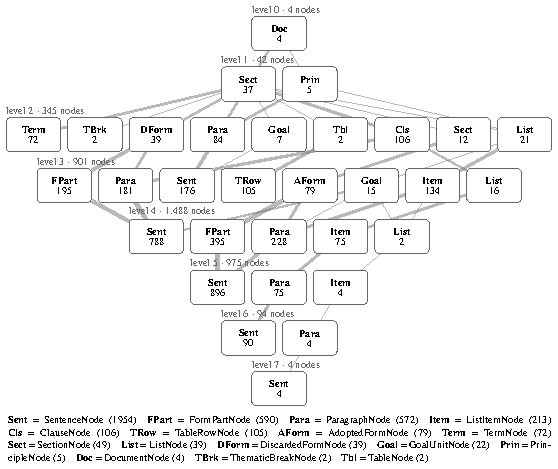
\includegraphics[width=\textwidth]{figures/f05/f05-graph-structure.pdf}
\caption{The containment tree of the corpus, aggregated to one chip per depth and node type. Each chip states the type abbreviation and its count at that depth; each line is the set of containment edges between two chips, drawn with a width proportional to the square root of the number of edges it carries. The row totals on the left sum to the 3{,}853 source nodes. The layout algorithm uses barycenter sweeps to place the groups without manual adjustment. The drawing aggregates: it shows where the corpus is deep and where it is wide, and it identifies no individual node.}
\label{fig:graph-structure}
\end{figure*}

The boundary between deterministic work and model-assisted work is drawn inside the pipeline and not around it. Figure~\ref{fig:pipeline} places it. Reading bytes, parsing CommonMark, building the typed intermediate representation, validating it, persisting it in one transaction, and running the link passes are pure functions of their input, with no model call and no database read. A model is invoked at one stage only, on one bounded unit at a time, under a pinned prompt, and its answer must satisfy a versioned schema before anything accepts it.

Six operations are closed to a model by construction. A model never assigns an identity, never parses structure, never resolves a cross-reference, never extends the controlled vocabulary, never evaluates a rule against a project state, and never decides a finding or a reachability answer. What a model contributes is an interpretation of one sentence, offered in a fixed shape. What turns interpretations into a recorded result is code and review together: code alone validates, canonicalizes, and persists them, and the semantic relations of the next subsection passed a review chain as well. The division matters for reproducibility. The deterministic stages replay from the source bytes at any time, and only the interpreted layer needs its recorded provenance to be trusted.

\begin{figure*}[t]
\centering
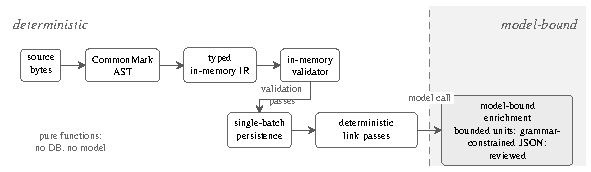
\includegraphics[width=\textwidth]{figures/f06/f06-ingestion-pipeline.pdf}
\caption{The ingestion pipeline and its determinism boundary. Left of the dashed line every stage is a pure function of its input, with no model call. The single model-bound stage on the right is entered one bounded unit at a time, with grammar-constrained output, a consensus check during calibration, and delegated review in production. The figure locates the boundary; the measurement methods and rebuild checks are in Appendix~\ref{app:repro}.}
\label{fig:pipeline}
\end{figure*}

The obvious alternative is to stop deriving and start authoring: write the rules in a formal language once, and generate the prose from them. That fails on the population this paper reports. Of 572 requirement units, 212 produced a classified gap rather than a proposition, mostly because the sentence names a concept the controlled vocabulary does not carry. A formal-first corpus would have had to either invent those concepts or leave the sentences out, and a sentence left out of the formal layer is a requirement with no record of its absence. Deriving from prose keeps the unrepresentable parts visible as counted gaps instead of absorbing them into a vocabulary that was never asked to cover them.

\subsection{Extraction and relation review}

Extraction ran over all 572 requirement units under one named single-lane evidence policy, with review and ratification delegated to an AI model. It compiled 360 of them and recorded a classified gap for the other 212, most of which name a concept the ratified vocabulary does not hold. Section~\ref{sec:method} states the fingerprint rule that governed calibration, and Section~\ref{sec:results} reports what the pass produced; this subsection states which passes ran under which policy.

Two things must not be confused at this stage. The controlled vocabulary is human work: I reviewed the candidate symbol registry symbol by symbol and ratified it on 2026-08-31, and no model may add to it afterwards. The semantic relations are not human work: they were proposed by a model, reviewed under delegated authority, and adjudicated by rule. Every artifact records which of the two it is, in its own metadata, so the standing of a number is read from the artifact and not from its surroundings.

Three relation passes produced the retained semantic edges, and the endpoint rules of each were frozen before it ran. The clause-to-goal pass put all 2{,}332 clause and goal-unit pairs to the lane, reviewed every answer case by case, and wrote 331 clause-to-goal links. The dependency pass covered the remaining 42{,}400 candidate pairs in 191 tiles and proposed 240 edges. A blind review of the 369 consequential answers, an adjudication that wrote 22 reusable rules, three judging rounds, and two seeded negative audits reduced those to 170 and overturned 75 pass answers. Two further rulings then judged the mutual pairs as pairs and the one remaining ring as a whole, removing 13 more and leaving 157 dependency links.

The candidate sets are checked as sets, not counted. The eligibility matrix is pinned by hash, and the two selections are derived from the frozen endpoint rule. The analysis layer refuses to call dependency coverage complete unless the registered passes cover the 44{,}732 candidates jointly and without overlap. Coverage of a candidate set is not correctness of its classifications, and the layer reports the two separately.

The two-stage shape is the one Section~\ref{sec:method} describes. Stage one calibrated the policy under dual-lane consensus on a ratified oracle and locked it. Stage two ran the corpus under reduced controls, with each pass carrying its own named policy and its own layered review. The tightening that would close the formal gate is a second production lane, and I deferred it on 2026-09-16 for time and budget reasons. The deferral changes no criterion. Every corpus-scale relation in this paper is delegated-AI single-lane evidence, and none of it is offered as dual-lane consensus or as human ratification.

\subsection{Deterministic analysis and change impact}

Five analysis operations read the graph without changing it. Verification runs the static checks over one database. Change-impact analysis partitions the corpus around a proposed edit. Change planning diffs two databases, or applies a mutation document to one, and emits the minimal ordered edit list. Derived export writes the coverage artifacts with a hash manifest. Source-change analysis compares the saved graph against the current source files. Every operation binds its output to its input through a database identity block. That block carries the file digest, the schema version, the corpus digest, the evidence policies, and both the recorded and the recomputed graph fingerprints. Repeated runs produce byte-identical output.

Verification runs seventeen named checks in four families. Integrity checks read the database itself: foreign keys, overall database integrity, dangling edge endpoints, duplicate relation edges, invalid endpoint types, and the validity of every stored rule against its schema. Coverage checks read the corpus: clauses with no implementing path, goal units with no inbound path, and the totals of the classified gaps. Consistency checks read the propositions: dangling condition references, directed cycles, and deontic clashes between an obligation and a prohibition whose guards can both hold. Provenance checks read the evidence: relation-edge provenance, the consistency of decisions with edges, the presence of dependency evidence, the incremental record, and authority leakage. The deterministic checks on defined terms follow the requirements-smell tradition \citep{femmer2017}, and the goal-coverage check descends from goal-oriented requirements analysis \citep{vanlamsweerde2001}.

Change impact analysis \citep{kretsou2021} is answered here as a partition and not as a list. The eligible universe is every source node. The seed nodes identify the elements selected for the proposed edit. Everything reachable from a seed over a propagating edge type, within the depth cap, is what the change may affect, and each entry carries its minimum depth over those edge types and a witness path whose steps record their direction. The rest of the universe is either proven unaffected or reported as blocked. Containment and document order do not propagate, because position in a document is not coupling.

A node enters the unaffected set only when two facts both hold. Dependency coverage must be complete, which establishes that every eligible dependency candidate in the defined universe has been classified under the registered policy, and the frontier must not be truncated, which establishes that the walk ended naturally rather than at the cap. Coverage alone is not enough: a walk cut short leaves the nodes past the frontier unexamined, and an unexamined node has not been proven to be anything. While either fact fails, the unaffected set is empty and every unreached node is reported as blocked. The rule is what stops the analysis from issuing a clearance it cannot support.

One change makes the behaviour concrete. Clause \hyperlink{nss-16.2}{16.2} of the Specification is the clause that makes the minimum check set mandatory, and Section~\ref{sec:standard} states that it names 24 grounds. A proposal to change it is seeded on that clause alone, and the analysis is run against the frozen dependency database at increasing depth caps. At depth 1 it reaches 45 nodes. At depth 2 it reaches 185, among them 94 of the 106 clauses, 30 of the 79 adopted forms, 13 goal units, and 4 of the 5 principles. At depth 4 it reaches 581, and the frontier is still truncated, so nothing is cleared. At depth 8 the walk converges: 1 node must change, 762 may be affected, 3{,}090 are proven unaffected under the recorded dependency graph, none are blocked, and the frontier is not truncated.

The converged answer is honest and of low discriminating value, and the reason is a property of this corpus rather than a defect of the method. The propagating graph is dominated by one large component, so a deep walk from almost any clause saturates it, and three unrelated seeds converge on the same 762 nodes. What the converged run establishes is the complement: 3{,}090 nodes lie outside the component and cannot be reached from this clause at any depth.

The useful reading is at the shallow depths, and the edge types that enter each depth say where it stops being useful. Every one of the 45 nodes at depth 1 is entered by a relation the clause itself asserts: 24 by its grounds, 15 by a recorded dependency, and 6 by an implementing link. The 140 added at depth 2 are entered the same way, by 66 implementing links, 44 explicit cross-references, 43 grounds, and 33 dependencies, and by nothing else; a node can be entered by more than one type. At depth 3 shared vocabulary appears, and at depth 4 it dominates: 236 of the 265 nodes added there are entered because two sentences use the same defined term. Two sentences that share a term are not thereby coupled. The depth-2 set of 185 is therefore the last one every member of which is reached by an asserted relation or an explicit reference, which is what makes it the review list rather than an arbitrary cut. The converged set stays useful as the outer boundary of what could ever matter.

Source-change analysis answers the same question from the other end. It compares the saved document bytes with the current files and reparses in memory. It reruns the term, reference, and appendix checks, and reports which findings are new and which are resolved. It identifies added, removed, and modified units from their full extents, and seeds the impact walk with those units and with the targets of the links inside them. A line shift alone changes nothing. The scope of its answer is stated in the report as the saved graph only, and any non-empty source difference sets a review flag, because a new dependency cannot be proven from old evidence. An unaffected verdict in the baseline partition is not a clearance for new meaning.

Change planning closes the loop by producing the edit rather than the diagnosis. Its input is a baseline and a candidate, or a baseline and a mutation document. It emits a deterministic ordered list of edit operations in a fixed group order. It also maps which findings the change introduces and which it resolves, and seeds a blast-radius run on the changed nodes. A locked regression fixture holds the method to that contract. For a goal deliverable with no inbound implementing path, the expected plan is exactly one added edge. The test replays that operation onto a scratch copy and reruns verification, and the targeted finding is resolved with no new error.

The practical result is the inspection path. When a clause changes, the traversal names the clauses that share its grounds, the adopted forms it descends from, the goal units it serves, the propositions extracted from it, and the terms it uses. Those are the contracts to reread, the records to reissue, and the checks to rerun. The list is produced by a query rather than by memory, it is the same list for every reader, and each entry carries the path that put it there.

\begin{figure*}[t]
\centering
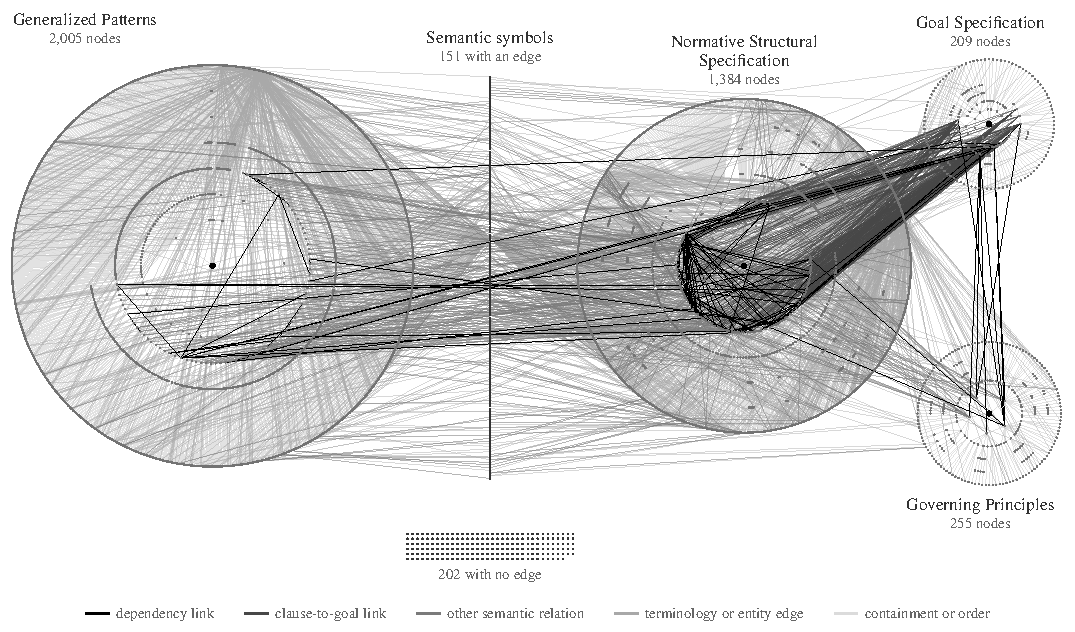
\includegraphics[width=\textwidth]{figures/f07/f07-semantic-graph.pdf}
\caption{The semantic graph in full: every one of the 4{,}206 nodes and every edge of the dependency database, recomputed 2026-09-21. No reduction is applied. Each document is one radial tree, and the area of each tree is proportional to its node count. Every leaf sits on the rim of its tree in document order, and each internal node sits at the mean angle of its children at a radius set by its depth, so containment reads as the spokes of a tree and document order as its rim. The Normative Structural Specification, which holds most of the relations, stands between Generalized Patterns and the two small documents, Governing Principles and the goal document. The 151 semantic symbols that carry an edge form the column between Generalized Patterns and the Specification, ordered by the mean height of their neighbours; the 202 that carry none form the grid below it, being the 157 actions the schema stores as proposition fields rather than as edges and 45 further ratified symbols that no proposition refers to. Structural and reviewed semantic edges are separated by gray tone, as the key shows: dependency links solid black, clause-to-goal links dark gray, other semantic relations middle gray, terminology and entity edges light gray, and containment and ordering edges the lightest gray. The 8{,}913 directed edges render as 8{,}905 undirected lines, because eight parallel pairs collapse into one line each. The relation edges are delegated-AI single-lane output under the review conditions described in Appendix~\ref{app:repro}: not human ratification, not dual-lane consensus, and not a closed gate.}
\label{fig:semantic-graph}
\end{figure*}

\subsection{Implemented checks and remaining limits}

The analysis used three successive databases: the extraction database, the relation database, and the dependency database. What each operation can conclude depends on which stage it reads. The first two lack complete dependency evidence, so their change-impact results clear no node as unaffected. The third records both relation passes and supplies the final dependency and verification results. Appendix~\ref{app:repro} states the input stage for each measurement. Verification passes on the dependency database under a ruling that lowers the 39 conflicts to informational severity and leaves them visible.

What stays open is reported rather than repaired, and nothing is closed by relabelling. Uncovered clauses, uncovered goal units, and extraction gaps all stay in the report at warning or informational severity. Four directed cycles stand by decision rather than by oversight, because the corpus states a mechanism and its own change control in one clause, and a rule that governs its own amendment is a cycle a reader should see. Section~\ref{sec:results} reports each finding against the artifact and the policy that produced it.

One implemented check has no active restrictions to enforce. Authority leakage is implemented and runs on every verification, and it reports nothing, because the ratified registry declares an empty actor-action binding list under an unrestricted policy. An empty list imposes no restriction, so the check has nothing to enforce. The twenty bindings a generator derived are benchmark evidence and not an authority matrix: they cover twenty of the 1{,}099 possible pairs of 7 actors and 157 actions, leave most actors unbound, and carry no clause-level provenance. Until a complete matrix is approved by a human, authority enforcement is specified and not active, and this paper claims it as neither.

The reserved work is therefore of two kinds. One is evidence: a second production lane would let the corpus-scale relations be reported as dual-lane consensus instead of reviewed single-lane output, and that gate stays open by decision. The other is capability: the authority matrix, and a scope repair that would let the 39 clashes be re-extracted rather than settled by ruling. Both are named as open in the project record, with the criteria that would close them unchanged.

The checker's schedule binds the checker and binds nothing else. The Specification requires a project to run a minimum set of sixteen normative checks over its own record, and Section~\ref{sec:standard} states that requirement and its deviation rule. Those checks are obligations on a project, and they are satisfied by whatever the project uses to run them. A check that this checker has not yet implemented is not a check a project may skip. The two sets are about different subjects: the checks reported in this section read four documents, and the checks the Specification mandates read a project record.


Figure~\ref{fig:semantic-graph} draws the whole graph at once, and its purpose is to connect the source model of this section to the analyses above it. The spokes are the containment tree that the parser produced deterministically from the bytes. The darker chords are the relations a model proposed and a review chain accepted. Reading the two classes apart is the point of the drawing: the structure is replayable from the source at any time, and the semantics carry the standing of the policy that produced them. Section~\ref{sec:results} reports what the checks found in that graph.
